\documentclass[11pt,a4paper]{article}

\usepackage[utf8]{inputenc}
\usepackage{amsmath, amssymb, amsthm}
\usepackage{geometry}
\usepackage{hyperref}
\usepackage{mathrsfs}
\usepackage{graphicx}
\usepackage{xcolor}

\geometry{margin=1in}

\title{\Large \textbf{Multidimensional Tensor Convolution\\ and the Spectral Cutoff of Lattice Transitions}}
\author{Ruqing Chen\\
\small GUT Geoservice Inc., Montreal, Quebec, Canada\\
\small \texttt{ruqing@hotmail.com}}
\date{\today}

\newtheorem{theorem}{Theorem}
\newtheorem{corollary}{Corollary}
\newtheorem{lemma}{Lemma}
\newtheorem{definition}{Definition}

\begin{document}

\maketitle

\begin{abstract}
Transitioning from the single-frequency phase space ($\mathbb{T}^1$) explored in Parts XX and XXI, this paper escalates the Arithmetic Geodynamics framework to the multidimensional product space $\prod_{q>3}\mathbb{T}^1_q$. We investigate the superposition of congruence interference across all prime frequencies. We discover a profound analytic behavior: for any fixed spatial translation $j$, constructive low-frequency interference ($O(1/q)$ deviation) is strictly confined to a finite set of primes dividing $j$ or its linear derivatives. Consequently, the infinite high-frequency tail is deterministically locked into a destructive interference state bounded by $O(1/q^2)$, guaranteeing absolute Euler convergence to a strictly positive constant. This enables the precise formulation of the Spectral Cutoff $k^\star(\varepsilon)$ and the construction of the universal Spatial Transition Operator for the 6N lattice.
\end{abstract}

\section{Introduction}
In Parts XX and XXI, we modeled the spatial entanglement of prime constellations at a single spatial frequency $q$ using circular convolution integrals on $\mathbb{T}^1$~\cite{ChenXX,ChenXXI}. We mapped the $\mathrm{dead}(q)$ mechanism to geometric indicator functions, yielding quantized interference states.

However, the physical reality of the 6N lattice is that a constellation center $N$ is simultaneously bombarded by the congruence waves of \textit{all} prime frequencies $q > 3$. To compute the absolute joint survival probability of two centers separated by distance $j$, we must ascend to a high-dimensional phase-space tensor product and evaluate the global spatial correlation $R(j)$. This necessitates a rigorous proof of spectral decay to define a practical truncation boundary.

\section{Ascension to Multidimensional Tensor Space $\mathbb{T}^\infty$}

Since the modular residues of distinct primes are asymptotically independent (by the Chinese Remainder Theorem limit as $X \to \infty$), the global phase space is the Cartesian product of individual frequency tori:
\begin{equation}
\mathcal{T} = \prod_{q > 3} \mathbb{T}^1_q
\end{equation}

The global spatial correlation ratio $R(j)$ between two constellations (e.g., Twin-Twin) is the infinite product of the single-frequency circular convolution integrals $R_q(j)$ derived in Part XX:
\begin{equation}
R(j) = \prod_{q > 3}^{\infty} R_q(j)
\end{equation}

\section{Absolute Convergence and Finite Resonance}

A fundamental challenge in analytic number theory is proving the absolute convergence of infinite products. If the interference amplitude $|R_q(j) - 1|$ decays only as $O(1/q)$, the product diverges. We must examine the asymptotic behavior of the three quantized interference states.

Recall the Twin-Twin convolution states from Part XX~\cite{ChenXX}:
\begin{itemize}
    \item \textbf{State A (Constructive):} $R_q(j) = \frac{q}{q-2} \approx 1 + \frac{2}{q}$
    \item \textbf{State B (Partial):} $R_q(j) = \frac{q(q-3)}{(q-2)^2} \approx 1 + \frac{q-4}{(q-2)^2} \sim O(1/q)$
    \item \textbf{State C (Destructive):} $R_q(j) = \frac{q(q-4)}{(q-2)^2} = \mathbf{1 - \frac{4}{(q-2)^2}} \sim \mathbf{O(1/q^2)}$
\end{itemize}

\begin{theorem}[Finiteness of Constructive Resonance]
For any fixed spatial interval $j$, the $O(1/q)$ amplitude states (States A and B) can only be triggered by a strictly finite number of prime frequencies.
\end{theorem}
\begin{proof}
State A requires $j \equiv 0 \pmod q$, which implies $q \mid j$. 
State B requires $j \equiv \pm 3^{-1} \pmod q \implies 3j \pm 1 \equiv 0 \pmod q$, which implies $q \mid (3j \pm 1)$.
Since $j$ is a fixed finite integer, the integers $j$ and $3j \pm 1$ possess a strictly finite number of prime factors. Thus, there exists a threshold frequency $q_{max} \le 3j+1$ beyond which States A and B can never occur.
\end{proof}

\begin{corollary}[Absolute High-Frequency Convergence]
For all primes $q > 3j+1$ (where $q \ge 5$), the geometric entanglement is deterministically locked into State C. The remaining infinite product is $\prod_{q > 3j+1} \left(1 - \frac{4}{(q-2)^2}\right)$. Since $\sum \frac{1}{q^2}$ converges, and each term satisfies $1 - \frac{4}{(q-2)^2} \ge \frac{5}{9} > 0$, the global correlation product $R(j)$ converges absolutely to a strictly positive constant. The interference acts as a quasi-periodic diffraction pattern dominated by small primes, not a divergent noise field.
\end{corollary}

\section{The Spectral Cutoff Constant $k^\star(\varepsilon)$}

Because the high-frequency tail converges rapidly via $O(1/q^2)$, the congruence interference pattern behaves analogously to a rapidly decaying Fourier spectrum. We can formally truncate this infinite product without loss of macroscopic physical fidelity.

\begin{definition}[Spectral Cutoff]
For a desired computational precision $\varepsilon > 0$ and spatial shift $j$, the spectral cutoff $k^\star$ is defined as the smallest index such that the tail product satisfies:
\begin{equation}
\left| 1 - \prod_{k = k^\star + 1}^{\infty} R_{p_k}(j) \right| < \varepsilon
\end{equation}
where $p_k$ is the $k$-th prime.
\end{definition}
This provides a rigorous analytic shortcut. Rather than computing infinite series to determine the spatial rippling of the $\mathrm{dead}(q)$ shield, one merely integrates over the first $k^\star$ dimensions of $\mathbb{T}^k$.

Evaluating the truncation numerically for the canonical case $j=1$ (all primes in State C, so the tail is the pure $O(1/q^2)$ floor) gives the cutoff explicitly. The full product is $R(1)=\prod_q R_q(1)=\mathfrak{S}_{\rm quad}/\mathfrak{S}_{\rm twin}^2=0.3969$, and the smallest cutoff prime $k^\star$ reaching relative precision $\varepsilon$ is:

\begin{table}[h]\centering
\begin{tabular}{ccc}
\hline
$\varepsilon$ & $k^\star$ & primes retained\\
\hline
$10^{-1}$ & $13$ & $4$\\
$10^{-2}$ & $73$ & $19$\\
$10^{-3}$ & $557$ & $100$\\
$10^{-4}$ & $4229$ & $577$\\
\hline
\end{tabular}
\caption{Spectral cutoff $k^\star(\varepsilon)$ for $R(1)$. To $1\%$ fidelity only
the primes up to $73$ are needed; the $O(1/q^2)$ tail makes the product converge
rapidly.}
\label{tab:kstar}
\end{table}

\begin{figure}[h]\centering
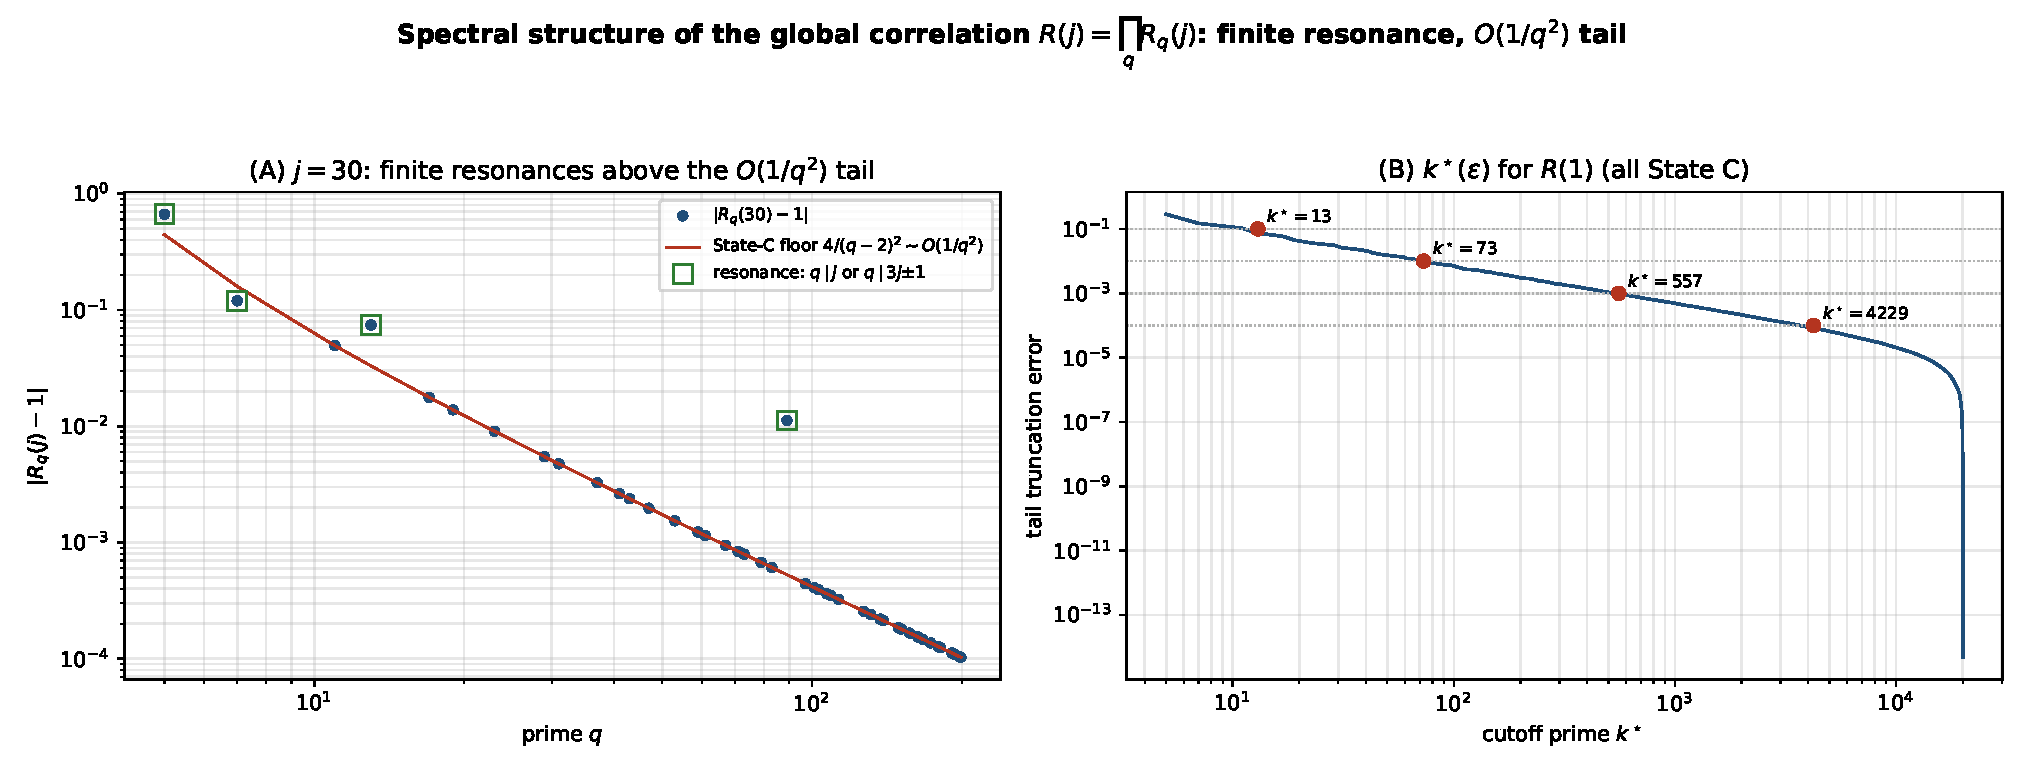
\includegraphics[width=0.97\textwidth]{fig_spectral_cutoff.pdf}
\caption{(A) For a fixed lag ($j=30$), the finitely many resonance primes
($q\mid j$ or $q\mid 3j\pm1$; here $5,7,13$) rise above the $O(1/q^2)$ State-C
floor $4/(q-2)^2$, on which every other prime sits exactly. (B) The resulting
truncation error of $\prod_{q\le k^\star}R_q(1)$ versus the cutoff prime
$k^\star$, with the $\varepsilon$ levels of Table~\ref{tab:kstar} marked.}
\label{fig:spectral}
\end{figure}

\section{The Spatial Transition Operator on the 6N Lattice}

With the global correlation tensor $R_{A,B}(j)$ absolutely convergent and computable via the $k^\star$ cutoff, we now formulate the universal macroscopic state transition. 

Let $S = \{S_1, S_2, \dots, S_n\}$ be the set of possible constellation states at any center (e.g., Twin, Empty, Triplet). Let $\rho_B$ be the base topological density of state $B$ (derived from integrating its continuous radial manifold $\ell$).

\begin{definition}[The Geodynamic Transition Operator]
Given that center $N$ is confirmed in state $A$, the conditional topological density of finding state $B$ at the translated center $N+j$ is given by the spatial operator $\mathcal{M}(j)$:
\begin{equation}
\rho(N+j = B \mid N = A) = \mathcal{M}_{A,B}(j) = \rho_B \cdot \prod_{q > 3}^{k^\star} R_{q, A, B}(j)
\end{equation}
\end{definition}

This Transition Operator extends beyond nearest-neighbour or Markovian models: the
correlation $R_{A,B}(j)$ does not decay with the lag $j$ but is quasi-periodic
(Part~XX), so the lattice carries a deterministic, long-range, small-prime-dominated
congruence correlation---structurally a multi-frequency diffraction grating rather
than a disordered field. We make no claim beyond this closed form: $\mathcal{M}(j)$
is the Hardy--Littlewood joint singular series re-expressed as a conditional density,
exact at integer lags and equal there to the discrete sieve ratio. It is a compact
bookkeeping of inter-centre correlation, not a dynamical or physical law.

\section{Conclusion}
By ascending to the product space $\prod_{q>3}\mathbb{T}^1_q$, we have shown the
absolute convergence of the global spatial correlation $R(j)=\prod_q R_q(j)$. The
mechanism is sharp: constructive resonance (States A, B, $O(1/q)$) is confined to
the finitely many primes dividing $j$ or $3j\pm1$, while the infinite tail is locked
in State C with $O(1/q^2)$ deviation, so the product converges to a strictly
positive constant and admits the spectral cutoff $k^\star(\varepsilon)$ of
Table~\ref{tab:kstar}. The resulting Spatial Transition Operator is a closed-form,
quasi-periodic bookkeeping of inter-centre correlation on the $6N$ skeleton---the
analytic completion of the diffraction picture of Volume~I. As throughout the
programme, the construction equals the discrete singular-series ratio at integer
lags, takes the Hardy--Littlewood heuristic as input, and makes no claim about the
infinitude of any constellation.

\paragraph{Data and code availability.}
The figure-generating script, the resonance-finiteness verifier, and the
$k^\star(\varepsilon)$ computation are openly available at
\url{https://github.com/Ruqing1963/6N-tensor-cutoff}~\cite{repo}.

\begin{thebibliography}{9}
\bibitem{HL} G.~H.~Hardy, J.~E.~Littlewood, \emph{Some problems of `Partitio
Numerorum'; III}, Acta Math.\ \textbf{44} (1923), 1--70.
\bibitem{ChenXVII} R.~Chen, \emph{Arithmetic geodynamics on the $6N$ skeleton}
(Part~XVII), Zenodo, doi:10.5281/zenodo.20541575 (2026).
\bibitem{ChenXX} R.~Chen, \emph{The circular convolution of prime constellations
in congruence phase space} (Part~XX), Zenodo, doi:10.5281/zenodo.20583994 (2026).
\bibitem{ChenXXI} R.~Chen, \emph{The irreducible three-body congruence correlation
and the annihilation lattice} (Part~XXI), Zenodo, doi:10.5281/zenodo.20584909 (2026).
\bibitem{Review} R.~Chen, \emph{Arithmetic geodynamics on the $6N$ skeleton: a
review of Parts I--XIX}, \url{https://github.com/Ruqing1963/6N-review} (2026).
\bibitem{repo} R.~Chen, \emph{Multidimensional tensor convolution and the spectral
cutoff of lattice transitions} (Part~XXII),
\url{https://github.com/Ruqing1963/6N-tensor-cutoff} (2026).
\end{thebibliography}

\end{document}